\documentclass[12pt,a4paper,oneside]{memoir}
\usepackage[T1]{fontenc}%necessario se si vuole il corretto funzionamento dell'algoritmo di costruzione dei capoversi
%pacchetto per la scelta dei font
\usepackage{cfr-lm}%Latin Modern esteso
\usepackage[utf8]{inputenc}%permette di inserire i caratteri nazionali
\usepackage[italian]{babel}
%impostazioni per l'italiano
\setISOcompliance
%\IntelligentComma
\usepackage{microtype}
\usepackage{parskip}
\frenchspacing
\setlength{\parindent}{0pt}
\usepackage{hyperref}
\usepackage{longtable}
\usepackage{array}
\usepackage{caption}
\usepackage[table,dvipsnames]{xcolor}
\definecolor{violetto}{RGB}{218,228,241}%prima riga tabelle
\definecolor{verdino}{RGB}{213,227,187}%colore box domande guida

% Don't forget to read the Memoir manual: memman.pdf

%%% Examples of Memoir customization
%%% enable, disable or adjust these as desired

%%% PAGE DIMENSIONS
% Set up the paper to be as close as possible to both A4 & letter:
\settrimmedsize{297mm}{210mm}{*}
\setlength{\trimtop}{0pt}
\setlength{\trimedge}{\stockwidth}
\addtolength{\trimedge}{-\paperwidth}
%\settypeblocksize{*}{\lxvchars}{1.618} % we want to the text block to have golden proportionals
%\setulmargins{50pt}{*}{*} % 50pt upper margins
%\setlrmargins{*}{*}{1.618} % golden ratio again for left/right margins
%\setheaderspaces{*}{*}{1.618}
\checkandfixthelayout 
%\settrimmedsize{297mm}{210mm}{*}
%\setlength{\trimtop}{0pt}
%\setlength{\trimedge}{\stockwidth}
%\addtolength{\trimedge}{-\paperwidth}
%\settypeblocksize{634pt}{448.13pt}{*}
%\setulmargins{4cm}{*}{*}
%\setlrmargins{*}{*}{1.5}
%\setmarginnotes{17pt}{51pt}{\onelineskip}
%\setheadfoot{\onelineskip}{2\onelineskip}
% This is from memman.pdf

%%% \maketitle CUSTOMISATION
% For more than trivial changes, you may as well do it yourself in a titlepage environment
\pretitle{\begin{center}\sffamily\huge\MakeUppercase}
\posttitle{\par\end{center}\vskip 0.5em}

%%% ToC (table of contents) APPEARANCE
\maxtocdepth{subsection} % include subsections
\renewcommand{\cftchapterpagefont}{}
\renewcommand{\cftchapterfont}{}     % no bold!

%%% HEADERS & FOOTERS
\pagestyle{ruled} % try also: empty , plain , headings , ruled , Ruled , companion

%%% CHAPTERS
\chapterstyle{hangnum} % try also: default , section , hangnum , companion , article, demo

\renewcommand{\chaptitlefont}{\Huge\sffamily\raggedright} % set sans serif chapter title font
\renewcommand{\chapnumfont}{\Huge\sffamily\raggedright} % set sans serif chapter number font

%%% SECTIONS
\hangsecnum % hang the section numbers into the margin to match \chapterstyle{hangnum}
\maxsecnumdepth{subsection} % number subsections

\setsecheadstyle{\Large\sffamily\raggedright} % set sans serif section font
\setsubsecheadstyle{\large\sffamily\raggedright} % set sans serif subsection font

%% END Memoir customization

\usepackage{calc}
\usepackage{multirow}%columns spanning several rows


\title{Piano Triennale dell'Offerta Formativa dell'Istituto Comprensivo Statale ``Don Milani''}
\author{}
\date{27/10/2016} % Delete this line to display the current date

\makeatletter
\newcommand{\rmnum}[1]{\romannumeral #1}%numeri romani minuscoli
\newcommand{\Rmnum}[1]{\expandafter\@slowromancap\romannumeral #1@}%numeri romani maiuscoli
\makeatother

\usepackage{graphicx}
\usepackage{epstopdf}
\DeclareGraphicsExtensions{.eps}

%%% BEGIN DOCUMENT
\begin{document}

%\maketitle
\tableofcontents* % the asterisk means that the contents itself isn't put into the ToC

\chapter*{Premessa}

\begin{itemize}
\item Il presente Piano triennale dell'offerta formativa, relativo all'Istituto Comprensivo Statale ``Don Lorenzo Milani'' di Misterbianco (CT), è elaborato ai sensi di quanto previsto dalla legge 13 luglio 2015, n. 107, recante la ``Riforma del sistema nazionale di istruzione e formazione e delega per il riordino delle disposizioni legislative vigenti'';
\item il piano è stato elaborato dal collegio dei docenti sulla base degli indirizzi per le attività della scuola e delle scelte di gestione e di amministrazione definiti dal dirigente scolastico con proprio atto di indirizzo comunicato durante la seduta del Collegio dei docenti del 29/09/2015;
\item il piano ha ricevuto il parere favorevole del collegio dei docenti nella seduta del 18/01/2016;
\item il piano è stato approvato dal consiglio d'istituto nella seduta del 20/01/2016;
\item il piano, dopo l'approvazione, è stato inviato all'USR competente per le verifiche di legge ed in particolare per accertarne la compatibilità con i limiti di organico assegnato
\item il piano è stato aggiornato dal collegio dei docenti nella seduta del 26/10/2016;
\item il piano aggiornato è stato approvato dal consiglio d'istituto nella seduta del 27/10/2016.
\end{itemize}

\chapter{Priorità strategiche}
Il presente Piano parte dalle risultanze dell'autovalutazione d'istituto, così come contenuta nel Rapporto di Autovalutazione (RAV), 
pubblicato sul sito web della scuola all'indirizzo:\\
\url{http://www.icsdonmilanimisterbianco.gov.it/}.\\

In particolare, si rimanda al RAV per quanto riguarda l'analisi del contesto in cui opera l'istituto, l'inventario delle risorse materiali, finanziarie, strumentali ed umane di cui si avvale, gli esiti documentati degli apprendimenti degli studenti, la descrizione dei processi organizzativi e didattici messi in atto.\\

Si riprendono qui in forma esplicita, come punto di partenza per la redazione del Piano, gli elementi conclusivi del RAV e cioè: priorità, traguardi di lungo periodo, obiettivi di processo.\\

\section{Priorità}
Le priorità si riferiscono agli obiettivi generali che la scuola si prefigge di realizzare nel lungo periodo attraverso l'azione di miglioramento. Le priorità che la scuola si pone devono necessariamente riguardare gli esiti degli studenti e, in questo ambito, il modello utilizzato per la stesura del RAV individua quattro aree obbligatorie --- risultati scolastici, risultati nelle prove standardizzate nazionali, competenze chiave e di cittadinanza, risultati a distanza --- e suggerisce di \textit{individuare un numero limitato di priorità (1 o 2) all'interno di una o due aree degli esiti degli studenti}.\\

Le priorità che l'Istituto si è assegnato per il prossimo triennio riguardano le seguenti aree:
\begin{enumerate} \label{priorità}
\item Risultati nelle prove standardizzate nazionali;
\item Competenze chiave e di cittadinanza.
\end{enumerate}

\section{Traguardi di lungo periodo}
I traguardi di lungo periodo riguardano i risultati attesi in relazione alle priorità strategiche. Si tratta di risultati previsti a lungo termine (3 anni). Essi articolano in forma osservabile e/o misurabile i contenuti delle priorità e rappresentano le mete verso cui la scuola tende nella sua azione di miglioramento. Per ogni priorità individuata deve essere articolato il relativo traguardo di lungo periodo.\\

I traguardi che l'Istituto si è assegnato in relazione alle priorità sono:
\begin{enumerate}
\item Ridurre la percentuale di alunni della scuola primaria presenti nei primi due livelli del 5\%, rispetto al dato nazionale, sia per la matematica, che per l'italiano;
\item Ridurre la percentuale di alunni della scuola secondaria di I grado presenti nei primi due livelli del 5\%, rispetto al dato nazionale, sia per la matematica, che per l'italiano;
\item Riduzione delle note disciplinari, del sei in comportamento, dei consigli di classe straordinari, di episodi problematici.
\end{enumerate}

Le motivazioni della scelta effettuata sono le seguenti:
\begin{enumerate}
\item Uniformità dei risultati tra le classi parallele, soprattutto per quanto riguarda l'italiano (sia primaria che secondaria);
\item Per la scuola secondaria di primo grado, diminuire il numero degli alunni presenti nei primi due livelli, sia per la matematica che per l'italiano;
\item Promozione di competenze sociali: senso di legalità e di un'etica della responsabilità, collaborazione e lo spirito di gruppo.
\end{enumerate}

\section{Obiettivi di processo}
Gli obiettivi di processo rappresentano una definizione operativa delle attività su cui si intende agire concretamente per raggiungere le priorità strategiche individuate. Essi costituiscono degli obiettivi operativi da raggiungere nel breve periodo (un anno scolastico) e riguardano una o più aree di processo.\\

Gli obiettivi di processo che l'Istituto ha scelto di adottare in vista del raggiungimento dei traguardi sono:
\begin{enumerate}
\item Progettare percorsi per competenze;
\item Elaborare e somministrare prove standardizzate. Elaborare criteri di correzione comuni;
\item Potenziare l'uso delle tecnologie in classe;
\item Realizzare attività laboratoriali finalizzate alla differenziazione dei percorsi didattici per gli studenti con maggiori difficoltà;
\item Promozione della figura del docente tutor per supportare gli studenti in difficoltà.
\end{enumerate}

La progettazione di percorsi per competenze, il potenziamento delle tecnologie in classe, l'istituzione del docente tutor per supportare gli studenti in difficoltà,  sono alcune delle azioni che, operando a largo raggio, confluiscono sinergicamente al raggiungimento delle priorità.\\

Le prove e i relativi criteri comuni di correzione saranno uno strumento di valutazione oggettiva.\\

Le competenze sociali saranno promosse da attività laboratoriali e di gruppo, sia curricolari che non, per sviluppare negli alunni il senso di appartenenza alla comunità scolastica, e condividerne le regole e i codici di comportamento, contribuendo a migliorare le competenze di cittadinanza.\\

\section{Risultati delle prove Invalsi e scelte conseguenti}

\subsection[Terze classi della scuola secondaria]{Risultati delle terze classi della scuola secondaria di primo grado nell'ultimo triennio}
L'analisi dei risultati di apprendimento nelle prove standardizzate nazionali di Italiano e Matematica delle terze classi della scuola secondaria di primo grado (tabelle \ref{invalsi13-14-iii}, \ref{invalsi14-15-iii}, \ref{invalsi15-16-iii} e le figure \ref{fig:distr-italiano-iii}, \ref{fig:distr-matematica-iii}), ha messo in luce i seguenti punti di forza:
\begin{itemize}
\item un progressivo miglioramento dei risultati nella prova di Matematica;
\item la distribuzione degli alunni nei livelli di apprendimento\footnote{Sulla base dei risultati su scala nazionale, l'INVALSI ha costruito 5 livelli di apprendimento:\\
Livello 1 punteggio minore o uguale al 75\% della media nazionale;\\
Livello 2 punteggio maggiore del 75\% e minore o uguale del 95\% della media nazionale;\\
Livello 3 punteggio maggiore del 95\% e minore o uguale del 110\% della media nazionale;\\
Livello 4 punteggio maggiore del 110\% e minore o uguale del 125\% della media nazionale;\\
Livello 5 punteggio maggiore del 125\% della media nazionale.} in Matematica è andata migliorando, con una diminuzione del numero degli alunni presenti nei livelli 1 e 2 e un aumento nei livelli 3 e 5.
\end{itemize}
Per quanto riguarda i punti di debolezza:
\begin{itemize}
\item in Italiano il numero degli alunni nel livello di apprendimento più basso è andato aumentando, mentre il numero degli alunni nel livello di apprendimento più alto è andato diminuendo;
\item i risultati in Italiano sono, in tutti e tre gli anni, inferiori rispetto alla media italiana.
\end{itemize}

\begin{table}[htp]
\caption{Risultati classi terze scuola secondaria di primo gr. a.s. 2013/14.} \label{invalsi13-14-iii}
\footnotesize
\begin{tabular}{|p{1.5cm}|p{1cm}|p{1cm}|p{1cm}|p{1cm}|p{1cm}|p{1cm}|p{1cm}|p{1cm}|}\hline
%\multicolumn{9}{|c|}{Risultati classi terze scuola secondaria di primo gr. a.s. 2013/14}\\\hline
\rowcolor{violetto}
&\multicolumn{4}{c|}{italiano}&\multicolumn{4}{c|}{matematica}\\\hline
\rowcolor{violetto}
i\-sti\-tu\-to clas\-se&p. medio&sicilia&sud e isole&italia&p. medio&sicilia&sud e isole&italia\\\hline
&&
$54,0$&
$55,5$&
$61,4$&&
$50,7$&
$51,2$&
$57,3$\\\hline
i\-sti\-tu\-to&
$59,1$&
\centering{$\Uparrow$}&
\centering{$\Uparrow$}&
\centering{$\Downarrow$}&
$46,8$&
\centering{$\Downarrow$}&
\centering{$\Downarrow$}&
\centering{$\Downarrow$}\tabularnewline\hline
\Rmnum{3} A&
$59,3$&
\centering{$\Uparrow$}&
\centering{$\Uparrow$}&
\centering{$\Downarrow$}&
$48,8$&
\centering{$\Leftrightarrow$}&
\centering{$\Downarrow$}&
\centering{$\Downarrow$}\tabularnewline\hline
\Rmnum{3} B&
$64,1$&
\centering{$\Uparrow$}&
\centering{$\Uparrow$}&
\centering{$\Uparrow$}&
$54,6$&
\centering{$\Uparrow$}&
\centering{$\Uparrow$}&
\centering{$\Downarrow$}\tabularnewline\hline
\Rmnum{3} C&
$66,9$&
\centering{$\Uparrow$}&
\centering{$\Uparrow$}&
\centering{$\Uparrow$}&
$27,3$&
\centering{$\Downarrow$}&
\centering{$\Downarrow$}&
\centering{$\Downarrow$}\tabularnewline\hline
\Rmnum{3} D&
$50,1$&
\centering{$\Downarrow$}&
\centering{$\Downarrow$}&
\centering{$\Downarrow$}&
$52,9$&
\centering{$\Leftrightarrow$}&
\centering{$\Uparrow$}&
\centering{$\Downarrow$}\tabularnewline\hline
\end{tabular}
\end{table}


\begin{table}[htp]
\caption{Risultati classi terze scuola secondaria di primo gr. a.s. 2014/15.} \label{invalsi14-15-iii}
\footnotesize
\begin{tabular}{|p{1.5cm}|p{1cm}|p{1cm}|p{1cm}|p{1cm}|p{1cm}|p{1cm}|p{1cm}|p{1cm}|}\hline
%\multicolumn{9}{|c|}{Risultati classi terze scuola secondaria di primo gr. a.s. 2014/15}\\\hline
\rowcolor{violetto}
&\multicolumn{4}{c|}{italiano}&\multicolumn{4}{c|}{matematica}\\\hline
\rowcolor{violetto}
i\-sti\-tu\-to clas\-se&p. medio&sicilia&sud e isole&italia&p. medio&sicilia&sud e isole&italia\\\hline
&&$54,2$&$55,9$&$60,3$&&$46,9$&$48,2$&$53,5$\\\hline
i\-sti\-tu\-to&
$52,2$&
\centering{$\Leftrightarrow$}&
\centering{$\Downarrow$}&
\centering{$\Downarrow$}&
$53,8$&
\centering{$\Uparrow$}&
\centering{$\Uparrow$}&
\centering{$\Leftrightarrow$}\tabularnewline\hline
\Rmnum{3} A&
$48,0$&
\centering{$\Downarrow$}&
\centering{$\Downarrow$}&
\centering{$\Downarrow$}&
$52,3$&
\centering{$\Uparrow$}&
\centering{$\Uparrow$}&
\centering{$\Downarrow$}\tabularnewline\hline
\Rmnum{3} B&
$59,1$&
\centering{$\Uparrow$}&
\centering{$\Uparrow$}&
\centering{$\Downarrow$}&
$59,7$&
\centering{$\Uparrow$}&
\centering{$\Uparrow$}&
\centering{$\Uparrow$}\tabularnewline\hline
\Rmnum{3} C&
$49,6$&
\centering{$\Downarrow$}&
\centering{$\Downarrow$}&
\centering{$\Downarrow$}&
$55,1$&
\centering{$\Uparrow$}&
\centering{$\Uparrow$}&
\centering{$\Uparrow$}\tabularnewline\hline
\Rmnum{3} D&
$52,7$&
\centering{$\Leftrightarrow$}&
\centering{$\Downarrow$}&
\centering{$\Downarrow$}&
$47,5$&
\centering{$\Leftrightarrow$}&
\centering{$\Leftrightarrow$}&
\centering{$\Downarrow$}\tabularnewline\hline
\end{tabular}
\end{table}

\clearpage

\begin{table}[htp]
\caption{Risultati classi terze scuola secondaria di primo gr. a.s. 2015/16.} \label{invalsi15-16-iii}
\footnotesize
\begin{tabular}{|p{1.5cm}|p{1cm}|p{1cm}|p{1cm}|p{1cm}|p{1cm}|p{1cm}|p{1cm}|p{1cm}|}\hline
%\multicolumn{9}{|c|}{Risultati classi terze scuola secondaria di primo gr. a.s. 2015/16}\\\hline
\rowcolor{violetto}
&\multicolumn{4}{c|}{italiano}&\multicolumn{4}{c|}{matematica}\\\hline
\rowcolor{violetto}
i\-sti\-tu\-to clas\-se&p. medio&sicilia&sud e isole&italia&p. medio&sicilia&sud e isole&italia\\\hline
&&$51,0$&$52,5$&$57,6$&&$43,9$&$43,1$&$48,1$\\\hline
i\-sti\-tu\-to&
$51,3$&
\centering{$\Leftrightarrow$}&
\centering{$\Leftrightarrow$}&
\centering{$\Downarrow$}&
$51,3$&
\centering{$\Uparrow$}&
\centering{$\Uparrow$}&
\centering{$\Uparrow$}\tabularnewline\hline
\Rmnum{3} A&
$56,0$&
\centering{$\Uparrow$}&
\centering{$\Uparrow$}&
\centering{$\Downarrow$}&
$50,5$&
\centering{$\Uparrow$}&
\centering{$\Uparrow$}&
\centering{$\Uparrow$}\tabularnewline\hline
\Rmnum{3} B&$41,3$&
\centering{$\Downarrow$}&
\centering{$\Downarrow$}&
\centering{$\Downarrow$}&
$49,3$&
\centering{$\Uparrow$}&
\centering{$\Uparrow$}&
\centering{$\Uparrow$}\tabularnewline\hline
\Rmnum{3} C&
$55,5$&
\centering{$\Uparrow$}&
\centering{$\Uparrow$}&
\centering{$\Downarrow$}&
$53,9$&
\centering{$\Uparrow$}&
\centering{$\Uparrow$}&
\centering{$\Uparrow$}\tabularnewline\hline
\end{tabular}
\end{table}

\begin{figure}[htp]
\centering
\caption{Distribuzione degli alunni delle classi terze scuola secondaria di primo grado per livelli di apprendimento nel triennio nella prova di italiano.}
\label{fig:distr-italiano-iii}
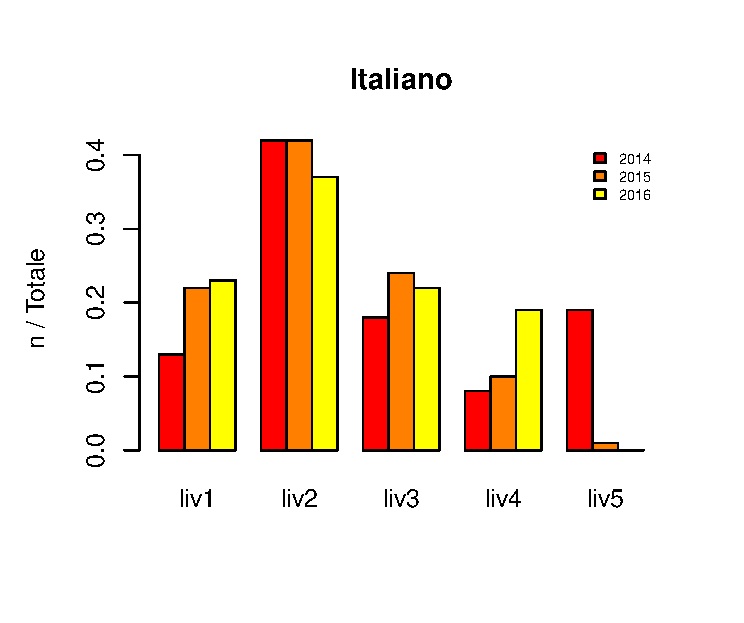
\includegraphics[width=0.8\linewidth]{italiano}
\end{figure}

\clearpage

\begin{figure}[htp]
\centering
\caption{Distribuzione degli alunni delle classi terze scuola secondaria di primo grado per livelli di apprendimento nel triennio nella prova di matematica.}
\label{fig:distr-matematica-iii}
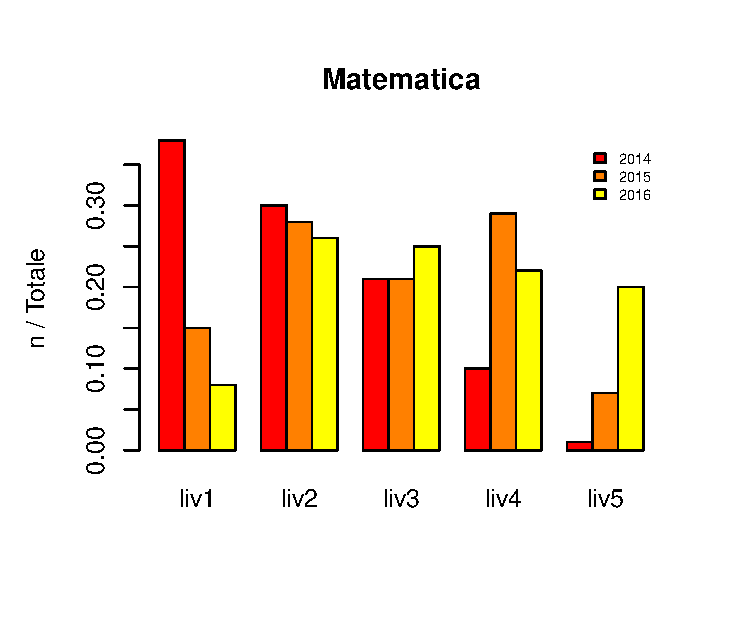
\includegraphics[width=0.8\linewidth]{matematica}
\end{figure}

\subsection[Seconde e quinte della scuola primaria]{Risultati delle seconde e delle quinte classi della scuola primaria nell'ultimo triennio}

I risultati relativi all'anno scolastico 2014/2015 non sono disponibili perché il numero degli alunni assenti alla prova ha superato il 50\% per ogni classe coinvolta nella prova. I risultati delle seconde relativi all'anno scolastico 2015/2016 non sono particolarmente significativi perché sono stati restituiti i dati di una sola classe su tre, a causa dell'elevato numero delle assenze.\\
L'analisi dei risultati di apprendimento nelle prove standardizzate nazionali di Italiano e Matematica delle seconde e quinte classi della scuola primaria (tabelle \ref{invalsi13-14-ii}, \ref{invalsi15-16-ii}, \ref{invalsi13-14-v} e \ref{invalsi15-16-v}), ha messo in luce i seguenti punti di forza:
\begin{itemize}
\item uniformità dei risultati tra le classi;
\item i risultati relativi all'anno scolastico 2013/2014 sono superiori anche alla media italiana.
\end{itemize}
Per quanto riguarda i punti di debolezza:
\begin{itemize}
\item per le quinte si nota una diminuzione dei punteggi dal 2013/2014 al 2015/2016 con risultati in quest'ultimo anno insufficienti rispetto alla media della Sicilia e anche relativamente a classi/scuole con background familiare simile;
\item per le quinte si nota una mancanza di uniformità nei risultati in Matamatica nell'anno scolastico 2015/2016;
\item i primi due livelli sono complessivamente più popolati rispetto alla media nazionale e di sud e isole sia per l'italiano  che per la matematica.
\end{itemize}

\`{E} opportuno precisare che una delle quattro classi quinte dell'anno scolastico 2015/2016, ha avuto un travagliato percorso didattico nei primi tre fondamentali anni della scuola primaria --- trasferimenti dei docenti, elevato numero di alunni svantaggiati, problematici e con scarse abilità di base --- tanto che si è operato un rimescolamento degli alunni delle sezioni A e B, tra il terzo ed il quarto anno. L'esito delle prove Invalsi, in particolare per la matematica, dimostra che non è stato possibile ridurre il divario con le altre classi, tuttavia dei miglioramenti sono stati riscontrati e, soprattutto, l'aver rilevato questa problematica, ha permesso di rivedere i criteri di formazione delle prime classi di ogni ciclo dal 2014/2015 in poi al fine di ridurre, quanto più possibile, la varianza tra le classi.  


\begin{table}[htp]
\caption{Risultati classi seconde scuola primaria gr. a.s. 2013/14.} \label{invalsi13-14-ii}
\footnotesize
\begin{tabular}{|p{1.5cm}|p{1cm}|p{1cm}|p{1cm}|p{1cm}|p{1cm}|p{1cm}|p{1cm}|p{1cm}|}\hline
%\multicolumn{9}{|c|}{Risultati classi seconde scuola primaria gr. a.s. 2013/14}\\\hline
\rowcolor{violetto}
&\multicolumn{4}{c|}{italiano}&\multicolumn{4}{c|}{matematica}\\\hline
\rowcolor{violetto}
i\-sti\-tu\-to clas\-se&p. medio&sicilia&sud e isole&italia&p. medio&sicilia&sud e isole&italia\\\hline
&&
$56,5$&
$58,3$&
$61,0$&&
$51,4$&
$53,1$&
$54,6$\\\hline
i\-sti\-tu\-to&
$75,7$&
\centering{$\Uparrow$}&
\centering{$\Uparrow$}&
\centering{$\Uparrow$}&
$66,5$&
\centering{$\Uparrow$}&
\centering{$\Uparrow$}&
\centering{$\Uparrow$}\tabularnewline\hline
\Rmnum{2} A&
$77,9$&
\centering{$\Uparrow$}&
\centering{$\Uparrow$}&
\centering{$\Uparrow$}&
$69,8$&
\centering{$\Uparrow$}&
\centering{$\Uparrow$}&
\centering{$\Uparrow$}\tabularnewline\hline
\Rmnum{2} B&
$74,0$&
\centering{$\Uparrow$}&
\centering{$\Uparrow$}&
\centering{$\Uparrow$}&
$55,7$&
\centering{$\Uparrow$}&
\centering{$\Uparrow$}&
\centering{$\Uparrow$}\tabularnewline\hline
\Rmnum{2} C&
$75,1$&
\centering{$\Uparrow$}&
\centering{$\Uparrow$}&
\centering{$\Uparrow$}&
$72,8$&
\centering{$\Uparrow$}&
\centering{$\Uparrow$}&
\centering{$\Uparrow$}\tabularnewline\hline
\end{tabular}
\end{table}

\begin{table}[htp]
\caption{Risultati classi seconde scuola primaria gr. a.s. 2015/16.} \label{invalsi15-16-ii}
\footnotesize
\begin{tabular}{|p{1.5cm}|p{1cm}|p{1cm}|p{1cm}|p{1cm}|p{1cm}|p{1cm}|p{1cm}|p{1cm}|}\hline
%\multicolumn{9}{|c|}{Risultati classi seconde scuola primaria gr. a.s. 2015/16}\\\hline
\rowcolor{violetto}
&\multicolumn{4}{c|}{italiano}&\multicolumn{4}{c|}{matematica}\\\hline
\rowcolor{violetto}
i\-sti\-tu\-to clas\-se&p. medio&sicilia&sud e isole&italia&p. medio&sicilia&sud e isole&italia\\\hline
&&
$44,9$&
$45,5$&
$48,2$&&
$48,7$&
$49,7$&
$51,0$\\\hline
i\-sti\-tu\-to&
$29,7$&
\centering{$\Downarrow$}&
\centering{$\Downarrow$}&
\centering{$\Downarrow$}&
$24,5$&
\centering{$\Downarrow$}&
\centering{$\Downarrow$}&
\centering{$\Downarrow$}\tabularnewline\hline
\Rmnum{2} A&
n.d.&
n.d.&
n.d.&
n.d.&
n.d.&
n.d.&
n.d.&
n.d.\tabularnewline\hline
\Rmnum{2} B&
$29,7$&
\centering{$\Downarrow$}&
\centering{$\Downarrow$}&
\centering{$\Downarrow$}&
$24,5$&
\centering{$\Downarrow$}&
\centering{$\Downarrow$}&
\centering{$\Downarrow$}\tabularnewline\hline
\Rmnum{2} C&
n.d.&
n.d.&
n.d.&
n.d.&
n.d.&
n.d.&
n.d.&
n.d.\tabularnewline\hline
\end{tabular}
\end{table}

\begin{table}[htp]
\caption{Risultati classi quinte scuola primaria gr. a.s. 2013/14.} \label{invalsi13-14-v}
\footnotesize
\begin{tabular}{|p{1.5cm}|p{1cm}|p{1cm}|p{1cm}|p{1cm}|p{1cm}|p{1cm}|p{1cm}|p{1cm}|}\hline
%\multicolumn{9}{|c|}{Risultati classi quinte scuola primaria gr. a.s. 2013/14}\\\hline
\rowcolor{violetto}
&\multicolumn{4}{c|}{italiano}&\multicolumn{4}{c|}{matematica}\\\hline
\rowcolor{violetto}
i\-sti\-tu\-to clas\-se&p. medio&sicilia&sud e isole&italia&p. medio&sicilia&sud e isole&italia\\\hline
&&
$53,9$&
$56,7$&
$61,0$&&
$56,7$&
$59,0$&
$62,9$\\\hline
i\-sti\-tu\-to&
$66,4$&
\centering{$\Uparrow$}&
\centering{$\Uparrow$}&
\centering{$\Uparrow$}&
$67,3$&
\centering{$\Uparrow$}&
\centering{$\Uparrow$}&
\centering{$\Uparrow$}\tabularnewline\hline
\Rmnum{5} A&
$62,7$&
\centering{$\Uparrow$}&
\centering{$\Uparrow$}&
\centering{$\Uparrow$}&
$63,0$&
\centering{$\Uparrow$}&
\centering{$\Uparrow$}&
\centering{$\Leftrightarrow$}\tabularnewline\hline
\Rmnum{5} B&
$69,6$&
\centering{$\Uparrow$}&
\centering{$\Uparrow$}&
\centering{$\Uparrow$}&
$60,4$&
\centering{$\Uparrow$}&
\centering{$\Leftrightarrow$}&
\centering{$\Downarrow$}\tabularnewline\hline
\Rmnum{5} C&
$68,6$&
\centering{$\Uparrow$}&
\centering{$\Uparrow$}&
\centering{$\Uparrow$}&
$78,1$&
\centering{$\Uparrow$}&
\centering{$\Uparrow$}&
\centering{$\Uparrow$}\tabularnewline\hline
\end{tabular}
\end{table}

\begin{table}[htp]
\caption{Risultati classi quinte scuola primaria gr. a.s. 2015/16.} \label{invalsi15-16-v}
\footnotesize
\begin{tabular}{|p{1.5cm}|p{1cm}|p{1cm}|p{1cm}|p{1cm}|p{1cm}|p{1cm}|p{1cm}|p{1cm}|}\hline
%\multicolumn{9}{|c|}{Risultati classi quinte scuola primaria gr. a.s. 2015/16}\\\hline
\rowcolor{violetto}
&\multicolumn{4}{c|}{italiano}&\multicolumn{4}{c|}{matematica}\\\hline
\rowcolor{violetto}
i\-sti\-tu\-to clas\-se&p. medio&sicilia&sud e isole&italia&p. medio&sicilia&sud e isole&italia\\\hline
&&
$57,8$&
$59,7$&
$63,5$&&
$45,7$&
$46,7$&
$51,0$\\\hline
i\-sti\-tu\-to&
$47,4$&
\centering{$\Downarrow$}&
\centering{$\Downarrow$}&
\centering{$\Downarrow$}&
$34,2$&
\centering{$\Downarrow$}&
\centering{$\Downarrow$}&
\centering{$\Downarrow$}\tabularnewline\hline
\Rmnum{5} A&
$56,3$&
\centering{$\Leftrightarrow$}&
\centering{$\Downarrow$}&
\centering{$\Downarrow$}&
$53,8$&
\centering{$\Uparrow$}&
\centering{$\Uparrow$}&
\centering{$\Uparrow$}\tabularnewline\hline
\Rmnum{5} B&
$40,2$&
\centering{$\Downarrow$}&
\centering{$\Downarrow$}&
\centering{$\Downarrow$}&
$24,1$&
\centering{$\Downarrow$}&
\centering{$\Downarrow$}&
\centering{$\Downarrow$}\tabularnewline\hline
\Rmnum{5} C&
$50,4$&
\centering{$\Downarrow$}&
\centering{$\Downarrow$}&
\centering{$\Downarrow$}&
$33,7$&
\centering{$\Downarrow$}&
\centering{$\Downarrow$}&
\centering{$\Downarrow$}\tabularnewline\hline
\Rmnum{5} D&
$44,0$&
\centering{$\Downarrow$}&
\centering{$\Downarrow$}&
\centering{$\Downarrow$}&
$32,7$&
\centering{$\Downarrow$}&
\centering{$\Downarrow$}&
\centering{$\Downarrow$}\tabularnewline\hline
\end{tabular}
\end{table}

\clearpage

\section{Scelte conseguenti}

%%%DA RIVEDERE COMPLETAMENTE

La mancanza/esiguità di fondi non ha consentito l'attivazione di corsi di recupero e di potenziamento extracurriculari , né il personale di potenziamento a disposizione ha potuto portare a termine quanto progettato  per il recupero e consolidamento delle abilità e delle conoscenze, in quanto spesso impegnato nella sostituzione dei docenti assenti (come previsto dalla L. 107). Le attività curriculari inerenti alla matematica del progetto  ``Con \ldots dividi''  hanno dato risultati positivi (come si evince dagli esiti Invalsi) , invece quelle inerenti all'italiano del progetto ``Il potere della parola'' hanno disatteso le aspettative , forse per la carenza di attività laboratoriali.

\section{Proposte e pareri provenienti dal territorio e dall'utenza}
Sono in corso continui contatti con gli altri istituti scolastici presenti nel territorio comunale e con l'ente locale per la realizzazione di alcuni interventi in particolare del settore relativo al diritto allo studio (educativa scolastica, finanziamento comodato d'uso libri di testo, interventi in genere relativi alla prevenzione del fenomeno della dispersione scolastica).


\chapter{Il Piano di Miglioramento}
Il Piano di Miglioramento si articola in 4 sezioni:
\begin{enumerate}
\item Scegliere gli obiettivi di processo più utili e necessari alla luce delle priorità individuate nella sezione 5 del RAV.
\item Decidere le azioni più opportune per raggiungere gli obiettivi scelti.
\item Pianificare gli obiettivi di processo individuati.
\item Valutare, condividere e diffondere i risultati alla luce del lavoro svolto dal Nucleo Interno di Valutazione.
\end{enumerate}
Le prime due sezioni permettono di documentare e condividere il percorso di problem solving messo in atto dalla scuola nella scelta degli obiettivi di processo e delle azioni di miglioramento ad essi connesse. Le sezioni 3 e 4, che costituiscono il cuore della progettazione del Piano di Miglioramento e del monitoraggio del suo andamento.

Ogni sezione è accompagnata da domande guida, utili per la compilazione del piano.


\section[Sezione 1. Scegliere gli obiettivi di processo]{Scegliere gli obiettivi di processo più rilevanti e necessari in tre passi (Sezione 1)}

Nella sezione 5 del RAV la scuola ha indicato alcuni obiettivi di processo che intende perseguire per raggiungere i traguardi connessi alle priorità. Per assicurarsi che la strada imboccata sia quella giusta la pianificazione del miglioramento riparte da qui: La scelta degli obiettivi è corretta? Sono questi gli obiettivi più utili alla promozione di un processo innovativo nella scuola? Sono connessi tra loro? E, soprattutto, la scuola si trova in condizioni oggettivamente favorevoli per la loro attuazione?


\subsection[Passo 1. Verificare la congruenza]{Verificare la congruenza tra obiettivi di processo e priorità/traguardi (Passo 1)}

Si chiede ora alla scuola di esplicitare la connessione tra ciascuno degli obiettivi di processo e le priorità individuate. Tale connessione deriva dal potenziale impatto che l'obiettivo potrà avere sul raggiungimento dei traguardi relativi alle priorità. In base a queste considerazioni, ogni obiettivo di processo può essere messo in relazione solo con una o con entrambe le priorità strategiche precedentemente identificate. In questo modo si ottiene un quadro sinottico degli obiettivi di processo, collegati alle priorità e ai traguardi.\\


\begin{center}
\fcolorbox{black}{verdino}{\hspace{5pt}%
\begin{minipage}[t]{.90\textwidth}

\vspace{1 em}

\textbf{Domande guida}\\

Ci sono nessi tra obiettivi e traguardi? se si, quali sono?\\
Ci sono ridondanze tra gli obiettivi individuati?\\
Gli obiettivi coprono tutti gli aspetti delle priorità dichiarate in modo efficace e completo?\\



\end{minipage}%
\hspace{5pt}
}
\end{center}


Nella Tabella \ref{obiettivi-e-priorità} vengono elencati gli obiettivi di processo, come indicati nella sezione 5 del RAV, e viene indicata con un ``SI'', nella colonna corrispondente al numero della priorità\footnote{Le due priorità sono state specificate a pagina \pageref{priorità}.} l'eventuale corrispondenza tra l'obiettivo e la priorità stessa.\\

\begin{table}[htp]
\caption{Relazione tra obiettivi di processo e priorità strategiche. Elencare gli obiettivi di processo come indicati nella sezione 5 del RAV e barrare le colonne 1 e/o 2 per indicare l'attinenza di ciascuno a una o entrambe le priorità.}  \label{obiettivi-e-priorità}
\footnotesize
\begin{tabular}{|>{\raggedright}p{4.cm}|>{\raggedright}p{5.9cm}|>{\raggedright}p{0.975cm}|>{\raggedright\arraybackslash}p{0.975cm}|}
\hline
\rowcolor{violetto}
Area di processo&Obiettivi di processo&\multicolumn{2}{c|}{Priorità \ldots}\\\cline{3-4}
\rowcolor{violetto}
&&1&2\\\hline
Curricolo, progettazione e valutazione&1 Progettare percorsi per competenze.&SI&\\\cline{2-4}
&2 Elaborare e somministrare prove standardizzate. Elaborare criteri di correzione comuni.&SI&\\\hline
Ambiente di apprendimento&1 Potenziare l'uso delle tecnologie in classe.&SI&\\\cline{2-4}
&2&&\\\hline
Inclusione e differenziazione&1 Realizzare attività laboratoriali finalizzate alla differenziazione dei percorsi didattici per gli studenti con maggiori difficoltà.&SI&SI\\\cline{2-4}
&2 Promuovere una figura di docente tutor per supportare gli studenti in difficoltà.&SI&\\\hline
\multirow{2}{35mm}{Continuità e orientamento}&1&&\\\cline{2-4}
&2&&\\\hline
Orientamento strategico e organizzazione della scuola&1 Revisione dei compiti affidati al personale docente, con particolare riferimento ai docenti coordinatori di classe.&&\\\cline{2-4}
&2&&\\\hline
Sviluppo e valorizzazione delle risorse umane&1 Aumentare la partecipazione dei docenti alle iniziative di formazione.&SI&SI\\\cline{2-4}
&2 Migliorare le ricadute delle attività di formazione nell'attività ordinaria della scuola.&SI&SI\\\hline
\multirow{2}{35mm}[3mm]{Integrazione con il territorio e rapporti con le famiglie}&\raisebox{1.6ex}[0cm][0cm]{1} \rule{0em}{3.5ex}&&\\\cline{2-4}
&\raisebox{1.6ex}[0cm][0cm]{2} \rule{0em}{3.5ex}&&\\\hline
\end{tabular}
\end{table}

\clearpage

\subsection[Passo 2. Elaborare una scala di rilevanza degli obiettivi di processo]{Elaborare una scala di rilevanza degli obiettivi di processo (Passo 2)}
Al fine di valutare la rilevanza di ciascuno degli obiettivi di processo, è importante compiere una stima della loro fattibilità. Ad ogni obiettivo si attribuisce un valore di fattibilità e uno di impatto, determinando una scala di rilevanza.\\

La stima dell'impatto implica una valutazione degli effetti che si pensa possano avere le azioni messe in atto al fine perseguire l'obiettivo descritto.\\

La stima della fattibilità si attua sulla base di una valutazione delle reali possibilità di realizzare le azioni previste, tenendo conto delle risorse umane e finanziarie a disposizione.\\

Si possono considerare i punteggi da 1 a 5 come segue:\\
1= nullo\\
2= poco\\
3= abbastanza\\
4= molto\\
5= del tutto\\

Il prodotto dei due valori fornisce una scala di rilevanza degli obiettivi di processo da mettere in atto.\\

Alla luce di queste valutazioni, la scuola può analizzare con più attenzione il peso strategico degli obiettivi di processo, in vista della pianificazione delle azioni ad essi sottese. In base ai risultati ottenuti la scuola può valutare se rivedere gli obiettivi dichiarati nel RAV, concentrandosi su quelli di rilevanza maggiore e, all'occorrenza, eliminare o ridimensionare il peso degli obiettivi di minore rilevanza.\\


\begin{center}
\fcolorbox{black}{verdino}{\hspace{5pt}%
\begin{minipage}[t]{.90\textwidth}

\vspace{1 em}

\textbf{Domande guida}\\

Ci sono obiettivi che, sebbene siano importanti, non è possibile realizzare?\\
Su quali obiettivi è opportuno concentrare le risorse a disposizione?\\



\end{minipage}%
\hspace{5pt}
}
\end{center}

\begin{table}[htp]
\caption{Calcolo della necessità dell'intervento sulla base di fattibilità ed impatto. Al fine di calcolare la rilevanza dell'obiettivo utilizzare la tabella riportando le stime sulla fattibilità e sull'impatto e il prodotto dei due valori numerici.}  \label{fattibilità-impatto-intervento}
\footnotesize
\begin{tabular}{|>{\raggedright}p{.67cm}|>{\raggedright}p{5.67cm}|>{\raggedright}p{1.195cm}|>{\raggedright}p{1.195cm}|>{\raggedright\arraybackslash}p{2.52cm}|}
\hline
\rowcolor{violetto}
&Obiettivo di processo elencati&Fat\-ti\-bi\-li\-tà (da 1 a 5)&Impatto (da 1 a 5)&Prodotto: valore che identifica la rilevanza dell'intervento\\\hline
1&Progettare percorsi per competenze.&4&4&16\\\hline
2&Elaborare e somministrare prove standardizzate. Elaborare criteri di correzione comuni.&4&4&16\\\hline
3&Potenziare l'uso delle tecnologie in classe.&4&4&16\\\hline
4&Realizzare attività laboratoriali finalizzate alla differenziazione dei percorsi didattici per gli studenti con maggiori difficoltà.&3&4&12\\\hline
5&Promuovere una figura di docente tutor per supportare gli studenti in difficoltà.&1&4&4\\\hline
6&Revisione dei compiti affidati al personale docente, con particolare riferimento ai docenti coordinatori di classe.&4&4&16\\\hline
7&Aumentare la partecipazione dei docenti alle iniziative di formazione.&2&4&8\\\hline
8&Migliorare le ricadute delle attività di formazione nell'attività ordinaria della scuola.&2&4&8\\\hline
\end{tabular}
\end{table}


\subsection[Passo 3. Ridefinire l'elenco degli obiettivi di processo e indicare i risultati attesi]{Ridefinire l'elenco degli obiettivi di processo e indicare i risultati attesi, gli indicatori di monitoraggio del processo e le modalità di misurazione dei risultati (Passo 3)}

Sulla base del lavoro precedente, la scuola può definire una lista ordinata degli obiettivi di processo, che saranno oggetto della successiva pianificazione.\\
Per ciascun obiettivo è necessaria una chiara definizione dei risultati attesi e degli indicatori su cui basare la misurazione periodica dei processi attivati, ai fini del monitoraggio dell'efficacia delle azioni intraprese. I risultati attesi e gli indicatori di processo devono essere espressi in una forma concreta e osservabile e saranno recuperati al momento del monitoraggio delle singole azioni.\\


\begin{center}
\fcolorbox{black}{verdino}{\hspace{5pt}%
\begin{minipage}[t]{.90\textwidth}

\vspace{1 em}

\textbf{Domande guida}\\

Quali sono gli obiettivi che s'intendono raggiungere nel prossimo anno scolastico?\\
Quali risultati ci si attende da ciascun obiettivo di processo scelto?\\
Quali indicatori dovranno essere utilizzati per capire se quella che si sta seguendo è la giusta direzione, al fine di raggiungere gli obiettivi previsti? In che modo  saranno misurati?\\



\end{minipage}%
\hspace{5pt}
}
\end{center}

\begin{footnotesize}
\captionsetup{width=13.5cm}
\begin{longtable}{|>{\raggedright}p{.342cm}|>{\raggedright}p{2.727cm}|>{\raggedright}p{2.727cm}|>{\raggedright}p{2.727cm}|>{\raggedright\arraybackslash}p{2.727cm}|}
\caption{Risultati attesi e  monitoraggio. Nella colonna ``indicatori di monitoraggio'' esprimere un elemento su cui basare il controllo periodico del processo in atto. L'indicatore dovrebbe essere un valore misurabile o comunque accertabile in modo univoco.} \label{risultati-e-monitoraggio}\\
\hline
\rowcolor{violetto}
&Obiettivo di processo in via di attuazione&Risultati attesi&Indicatori di monitoraggio&Modalità di rilevazione\\ \hline
\endfirsthead
\hline
\rowcolor{violetto}
&Obiettivo di processo in via di attuazione&Risultati attesi&Indicatori di monitoraggio&Modalità di rilevazione\\ \hline
\endhead
\hline \multicolumn{5}{r}{\emph{Continua nella pagina successiva}}
\endfoot
\hline
\endlastfoot
1&``Il potere della parola: evoluzione del lessico''.&Il miglioramento nella lettura, nella comprensione del testo, nella comunicazione orale, nella produzione scritta, nel lessico e nella metalinguistica.&Diminuire il numero di allievi nelle fasce L1 – L2 ($-5\%$: Dati INVALSI 2015-2016 sia per la scuola primaria che per la secondaria di I grado). 
Aumentare il numero di alunni nelle fasce L4 – L5 ($+5\%$: Dati INVALSI 2015-2016 sia per la scuola primaria che per la secondaria di $1^{\circ}$ grado).
Ridurre il numero di allievi gravemente&Raccolta dati sulla ricaduta delle azioni, da valutare in sede dipartimentale e di consiglio di classe (in itinere e finale);
somministrazione test di gradimento agli studenti e alle famiglie; somministrazione di prove comuni oggettive e criteri di correzione comuni; valutazione dei risultati delle prove invalsi.\\ \hline
&&&insufficienti al primo quadrimestre: $-25\%$.
Risultati delle prove INVALSI in italiano con un miglioramento degli esiti del $5\%$ nella differenza tra il risultato della scuola e la media nazionale e delle scuole con background simile. Somministrazione periodica di prove per classi parallele.&\\ \hline
2&``Con \ldots dividi''&Promuovere esperienze significative in cui gli strumenti matematici si mostrano sempre più utili per operare nella realtà.
Formulare ipotesi, controllare le conseguenze, progettare e sperimentare, discutere e argomentare le proprie scelte, raccogliere dati e costruire significati.&Diminuire il numero di allievi nelle fascia L2 ($-5\%$: Dati INVALSI 2015-16 solo per la prova Nazionale).
Diminuire il numero di allievi nelle fascia L1 ($-5\%$: Dati INVALSI 2015-16 scuola primaria).
Aumentare il numero di alunni nelle fasce L4 – L5 ($+5\%$: Dati INVALSI 2015-16 per la scuola primaria).&Raccolta dati sulla ricaduta delle azioni, da valutare in sede dipartimentale e di consiglio di classe (in itinere e finale); somministrazione test di gradimento agli studenti e alle famiglie; somministrazione di prove comuni oggettive e criteri di correzione comuni; valutazione dei risultati delle prove invalsi.\\ \hline
&&&Aumentare il numero di allievi nelle fascia L5 ($+5\%$: Dati INVALSI 2015-16 solo per la prova Nazionale).
Ridurre il numero di allievi gravemente insufficienti al primo quadrimestre : $-25\%$.
Risultati delle prove INVALSI in matematica con un miglioramento degli esiti nella scuola primaria del $5\%$ nella differenza tra il risultato della scuola e la media nazionale e un mantenimento della percentuale superiore nella Prova Nazionale.&\\ \hline
3&Coro, propedeutica musicale, nella scuola primaria&Allestimento di eventi canori e musicali, condivisione di regole e capacità di lavoro in gruppo&Riduzione delle assenze, degli ingressi in ritardo, delle note disciplinari, dei sei in comportamento, aumento del numero delle iscrizioni nell'indirizzo musicale.&Raccolta dati sulla ricaduta delle azioni, da valutare in sede di consiglio di classe (in itinere e finale);
somministrazione test di gradimento agli studenti e alle famiglie.\\ \hline
4&Formazione&Diffondere maggiormente la didattica laboratoriale riducendo i tempi della lezione frontale.
Incentivare l'uso delle nuove tecnologie in ambito didattico.&Incremento dell'uso della LIM nella didattica quotidiana (\mbox{$>1$} lezione settimanale).
Incremento dei docenti che sperimentano in aula le tecniche e gli strumenti suggeriti durante la formazione ($\ge50\%$).
Motivare l'apprendimento degli alunni attraverso l'uso delle nuove tecnologie legate alla didattica ($\ge50\%$ delle risposte positive al questionario).
Decremento delle insufficienze e delle gravi insufficienze: confronto con le prove in itinere durante il $2^{\circ}$ quadrimestre ($-25\%$).&Utilizzo delle piattaforme e-learning presenti nel sito della scuola, per la condivisione di materiale didattico da mettere a disposizione di tutti i docenti.
Raccolta dati sulla ricaduta indiretta delle azioni da valutare in sede dipartimentale e di consiglio di classe (in itinere e finale).
Somministrazione test di gradimento ai docenti in formazione e agli studenti.\\ \hline
\end{longtable}
\end{footnotesize}

\section[Sezione 2. Azioni per raggiungere ciascun obiettivo]{Decidere le azioni per raggiungere ciascun obiettivo di processo in due passi (Sezione 2)}

\subsection[Passo 1. Ipotizzare le azioni da compiere]{Ipotizzare le azioni da compiere considerandone i possibili effetti negativi e positivi a medio e a lungo termine (Passo 1)}

Decidere le azioni da compiere è un passaggio che richiede una riflessione attenta in termini di valutazione delle potenziali opportunità e rischi.\\
Occorre considerare che le azioni che si intraprenderanno potranno avere degli effetti positivi ma anche potenziali ricadute negative su altre dimensioni o attività nelle quali la scuola è impegnata.\\
È opportuno inoltre tenere presente che gli effetti delle azioni intraprese non si esauriranno nel breve periodo, ma avranno anche effetti di medio e lungo periodo.\\


\begin{center}
\fcolorbox{black}{verdino}{\hspace{5pt}%
\begin{minipage}[t]{.90\textwidth}

\vspace{1 em}

\textbf{Domande guida}\\

Quali sono gli effetti positivi che un'azione può produrre all'interno della scuola?\\
Quali sono invece gli aspetti negativi che la stessa azione può produrre, innescando meccanismi non virtuosi?\\
Queste azioni produrranno effetti anche i nei prossimi anni?\\


\end{minipage}%
\hspace{5pt}
}
\end{center}

\begin{table}[htp]
\caption{Valutazione degli effetti positivi e negativi delle azioni.}  \label{valutazioni-effetti-azioni}
\footnotesize
\begin{tabular}{|>{\raggedright}p{1.902cm}|>{\raggedright}p{2.337cm}|>{\raggedright}p{2.337cm}|>{\raggedright}p{2.337cm}|>{\raggedright\arraybackslash}p{2.337cm}|}
\hline
\rowcolor{violetto}
Azione prevista&Effetti positivi all'interno della scuola a medio termine&Effetti negativi all'interno della scuola a medio termine&Effetti positivi all'interno della scuola a lungo termine&Effetti negativi all'interno della scuola a lungo termine\\ \hline
1&con\-so\-li\-da\-men\-to delle capacità di comprensione e di rielaborazione del testo.&&Mi\-glio\-ra\-men\-to degli esiti scolastici e nelle prove INVALSI.&\\ \hline
2&Tradurre le situazioni reali in termini matematici e riconoscere gli schemi ricorrenti.&&Mi\-glio\-ra\-men\-to degli esiti scolastici e nelle prove INVALSI.&\\ \hline
3&Maggiore partecipazione alle attività scolastiche, diminuzione delle assenze.&&Maggiore motivazione all'apprendimento.&\\ \hline
4&Incremento dell'uso della LIM, sperimentazione di metodologie didattiche innovative.&&Maggiore motivazione degli alunni all'apprendimento.&\\ \hline	
\end{tabular}
\end{table}

\clearpage

\subsection[Passo 2. Rapportare gli effetti a un quadro di riferimento innovativo]{Rapportare gli effetti delle azioni a un quadro di riferimento innovativo (Passo 2)}

Le azioni pianificate avranno effetti duraturi se incideranno sul raggiungimento di obiettivi a breve termine, ma soprattutto se rappresenteranno un'occasione per avviare un profondo processo di innovazione e cambiamento della scuola.\\

Le azioni che s'intendono attivare vengono quindi messe in relazione con il quadro di riferimento che emerge dal lavoro che INDIRE svolge con le scuole delle Avanguardie Educative e si collega fortemente a quanto previsto dalla Legge 107/15 nota come ``Buona Scuola''.\\


\begin{center}
\fcolorbox{black}{verdino}{\hspace{5pt}%
\begin{minipage}[t]{.90\textwidth}

\vspace{1 em}

\textbf{Domande guida}\\

Le azioni possono essere connesse a qualcuno degli obiettivi previsti dalla Legge 107/15?\\
Le azioni prevedono modifiche agli ambienti di apprendimento e/o all'organizzazione scolastica?\\
Nelle azioni descritte si può riconoscere una linea di tendenza che porta verso l'innovazione?\\


\end{minipage}%
\hspace{5pt}
}
\end{center}

\begin{table}[htp]
\caption{Caratteri innovativi.}  \label{caratteri-innovativi}
\footnotesize
\begin{tabular}{|>{\raggedright}p{6.2572cm}|>{\raggedright\arraybackslash}p{6.2572cm}|}
\hline
\rowcolor{violetto}
Caratteri innovativi dell'obiettivo&Connessione con il quadro di riferimento di cui in Appendice A e B\\ \hline
1. Adeguamento dei codici comunicativi dei giovani ai differenti contesti: formale, non formale e informale&comma 7, lettera a) e p)\\ \hline
2. Verticalizzazione dell'attività laboratoriale&comma 7, lettera b) e p)\\ \hline
3. Arricchimento delle attività performative dell'orchestra dell'istituto&comma 7, lettera c)\\ \hline
4. La formazione dei docenti consentirà l'uso di metodologie didattiche tali da sollecitare la partecipazione attiva degli alunni nella costruzione del sapere e nella acquisizione delle competenze&comma 124 e punto n. 2 del Manifesto del movimento delle Avanguardie Educative (Sfruttare le opportunità offerte dalle ICT e dai linguaggi digitali per supportare nuovi modi di insegnare, apprendere e valutare)\\ \hline
\end{tabular}
\end{table}

\section[Sezione 3. Pianificare le azioni di ciascun obiettivo]{Pianificare le azioni di ciascun obiettivo di processo individuato in tre passi (Sezione 3)}

\subsection[Passo 1. Definire l'impegno delle risorse umane e strumentali]{Definire l'impegno delle risorse umane e strumentali (Passo 1)}

La pianificazione delle azioni è il cuore della predisposizione del piano. Si parte con la previsione dell'impegno di risorse umane interne alla scuola, definendo ciò che esula dalle normali funzioni di servizio e che ha un impatto aggiuntivo di carattere finanziario (docenti, personale ATA, DS) e di quelle esterne (consulenti, formatori, ecc.), quantificando le spese che la scuola intende sostenere per l'attuazione delle azioni descritte.\\

\begin{center}
\fcolorbox{black}{verdino}{\hspace{5pt}%
\begin{minipage}[t]{.90\textwidth}

\vspace{1 em}

\textbf{Domande guida}\\

Quali sono le risorse umane interne che la scuola ha a disposizione per raggiungere gli obiettivi di processo?\\
Quali sono le risorse umane esterne necessarie ad attivare i processi in modo efficace?\\
Quali sono le fonti finanziarie da cui la scuola intende attingere per coprire le spese necessarie?\\



\end{minipage}%
\hspace{5pt}
}
\end{center} 

\begin{table}[htp]
\caption{Descrivere l'impegno di risorse umane interne alla scuola.}  \label{descrivere-impegno-interno}
Obiettivo 1\\


\footnotesize
\begin{tabular}{|>{\raggedright}p{2.249851cm}|>{\raggedright}p{2.249851cm}|>{\raggedright}p{2.249851cm}|>{\raggedright}p{2.249851cm}|>{\raggedright\arraybackslash}p{2.249851cm}|}
\hline
\rowcolor{violetto}
Figure professionali&Tipologia di attività&Ore aggiuntive presunte&Costo previsto&Fonte finanziaria\\\hline
Docenti interni&Attività curricolare&Nessuna&$0,00$&\\\hline
Personale ATA&Attività curricolare&Nessuna&$0,00$&\\\hline
Altre figure&Nessuna&Nessuna&$0,00$&\\\hline
\multicolumn{5}{r}{\emph{Continua nella pagina successiva}}\\
\end{tabular}
\end{table}
\begin{table}[htp]
\normalsize{Obiettivo 2}\\

\footnotesize
\begin{tabular}{|>{\raggedright}p{2.249851cm}|>{\raggedright}p{2.249851cm}|>{\raggedright}p{2.249851cm}|>{\raggedright}p{2.249851cm}|>{\raggedright\arraybackslash}p{2.249851cm}|}\hline
\rowcolor{violetto}
Figure professionali&Tipologia di attività&Ore aggiuntive presunte&Costo previsto&Fonte finanziaria\\\hline
Docenti interni&Attività curricolare&Nessuna&$0,00$&\\\hline
Personale ATA&Attività curricolare&Nessuna&$0,00$&\\\hline
Altre figure&Nessuna&Nessuna&$0,00$&\\\hline
\end{tabular}

\vspace{1em}

\normalsize{Obiettivo 3}\\

\footnotesize
\begin{tabular}{|>{\raggedright}p{2.249851cm}|>{\raggedright}p{2.249851cm}|>{\raggedright}p{2.249851cm}|>{\raggedright}p{2.249851cm}|>{\raggedright\arraybackslash}p{2.249851cm}|}\hline
\rowcolor{violetto}
Figure professionali&Tipologia di attività&Ore aggiuntive presunte&Costo previsto&Fonte finanziaria\\\hline
Docenti interni&Attività curricolare&Nessuna&$0,00$&\\\hline
Personale ATA&Attività curricolare&Nessuna&$0,00$&\\\hline
Altre figure&Nessuna&Nessuna&$0,00$&\\\hline
\end{tabular}

\vspace{1em}

\normalsize{Obiettivo 4}\\

\footnotesize
\begin{tabular}{|>{\raggedright}p{2.249851cm}|>{\raggedright}p{2.249851cm}|>{\raggedright}p{2.249851cm}|>{\raggedright}p{2.249851cm}|>{\raggedright\arraybackslash}p{2.249851cm}|}\hline
\rowcolor{violetto}
Figure professionali&Tipologia di attività&Ore aggiuntive presunte&Costo previsto&Fonte finanziaria\\\hline
Docenti interni&Frequenza di incontri di formazione&$10$&$0,00$&\\\hline
Personale ATA&Attività curricolare&Nessuna&$0,00$&\\\hline
Altre figure: esperti esterni&Attività di formazione&$10$&$350,00$&\\\hline
\end{tabular}
\end{table}


\begin{table}[htp]
\caption{Descrivere l'impegno finanziario per figure professionali esterne alla scuola e/o beni e servizi.}  \label{descrivere-impegno-esterno}
\footnotesize
\begin{tabular}{|>{\raggedright}p{4.03092cm}|>{\raggedright}p{4.03092cm}|>{\raggedright\arraybackslash}p{4.03092cm}|}
\hline
\rowcolor{violetto}
Impegni finanziari per tipologia di spesa&Impegno presunto&Fonte finanziaria\\\hline
Formatori&Euro $350,00$&\\\hline
Consulenti&&\\\hline
Attrezzature&&\\\hline
Servizi&&\\\hline
Altro&&\\\hline
\end{tabular}
\end{table}

\clearpage

\subsection[Passo 2. Definire i tempi di attuazione]{Definire i tempi di attuazione delle attività (Passo 2)}

Al momento della progettazione ed anche ai fini del monitoraggio in una fase successiva, è importante definire una tempistica chiara dell'attuazione delle azioni pianificate. La tabella di pianificazione, per questo motivo, si configura come una vera e propria ``tabella di marcia'' da aggiornare in ogni momento, monitorando costantemente l'andamento del processo di miglioramento.\\

\begin{center}
\fcolorbox{black}{verdino}{\hspace{5pt}%
\begin{minipage}[t]{.90\textwidth}

\vspace{1 em}

\textbf{Domande guida}\\

È possibile fare una progettazione precisa delle azioni scandite nel corso dell'anno?\\
Chi è il responsabile del monitoraggio delle azioni affinché quel determinato obiettivo di processo sia in linea con i tempi?\\




\end{minipage}%
\hspace{5pt}
}
\end{center} 
\begin{table}[htp]
\caption{Tempistica delle attività}\label{tempistica-attività}
Obiettivo 1\\
Responsabile Prof.ssa Messina/Saitta\\

\footnotesize
\begin{tabular}{|>{\raggedright}p{2.4cm}|>{\raggedright}p{0.65cm}|>{\raggedright}p{0.65cm}|>{\raggedright}p{0.65cm}|>{\raggedright}p{0.65cm}|>{\raggedright}p{0.65cm}|>{\raggedright}p{0.65cm}|>{\raggedright}p{0.65cm}|>{\raggedright}p{0.65cm}|>{\raggedright}p{0.65cm}|>{\raggedright\arraybackslash}p{0.65cm}|}
\hline
\rowcolor{violetto}
Attività&\multicolumn{10}{l|}{Pianificazione delle attività}\\\hline
\rowcolor{violetto}
&1
Set&2
Ott&3
Nov&4
Dic&5
Gen&6
Feb&7
Mar&8
Apr&9
Mag&10
Giu\\\hline
Svolgimento delle attività con gli alunni&&&&&&x&x&x&&\\\hline
Monitoraggio&&&&&&&x&&x&\\\hline
Valutazione&&&&&&&&x&&x\\\hline
Dis\-se\-mi\-na\-zio\-ne&&&&&&&&&&x\\\hline
\multicolumn{11}{r}{\emph{Continua nella pagina successiva}}\\
\end{tabular}
\end{table}


\begin{table}[htp]
\normalsize{Obiettivo 2}\\
Responsabile Prof.ssa Strano\\

\footnotesize
\begin{tabular}{|>{\raggedright}p{2.4cm}|>{\raggedright}p{0.65cm}|>{\raggedright}p{0.65cm}|>{\raggedright}p{0.65cm}|>{\raggedright}p{0.65cm}|>{\raggedright}p{0.65cm}|>{\raggedright}p{0.65cm}|>{\raggedright}p{0.65cm}|>{\raggedright}p{0.65cm}|>{\raggedright}p{0.65cm}|>{\raggedright\arraybackslash}p{0.65cm}|}
\hline
\rowcolor{violetto}
Attività&\multicolumn{10}{l|}{Pianificazione delle attività}\\\hline
\rowcolor{violetto}
&1
Set&2
Ott&3
Nov&4
Dic&5
Gen&6
Feb&7
Mar&8
Apr&9
Mag&10
Giu\\\hline
Svolgimento delle attività con gli alunni&&&&&&x&x&x&&\\\hline
Monitoraggio&&&&&&&x&&x&\\\hline
Valutazione&&&&&&&&x&&x\\\hline
Dis\-se\-mi\-na\-zio\-ne&&&&&&&&&&x\\\hline
\end{tabular}

\vspace{1em}

\normalsize{Obiettivo 3}\\
Responsabile Ins. Pirri\\

\footnotesize
\begin{tabular}{|>{\raggedright}p{2.4cm}|>{\raggedright}p{0.65cm}|>{\raggedright}p{0.65cm}|>{\raggedright}p{0.65cm}|>{\raggedright}p{0.65cm}|>{\raggedright}p{0.65cm}|>{\raggedright}p{0.65cm}|>{\raggedright}p{0.65cm}|>{\raggedright}p{0.65cm}|>{\raggedright}p{0.65cm}|>{\raggedright\arraybackslash}p{0.65cm}|}
\hline
\rowcolor{violetto}
Attività&\multicolumn{10}{l|}{Pianificazione delle attività}\\\hline
\rowcolor{violetto}
&1
Set&2
Ott&3
Nov&4
Dic&5
Gen&6
Feb&7
Mar&8
Apr&9
Mag&10
Giu\\\hline
Svolgimento delle attività con gli alunni&&&&&x&x&x&x&&\\\hline
Monitoraggio&&&&&x&x&x&x&x&\\\hline
Valutazione&&&&&&&&x&&x\\\hline
Dis\-se\-mi\-na\-zio\-ne&&&&&&&&&&x\\\hline
\end{tabular}

\vspace{1em}

\normalsize{Obiettivo 4}\\
Responsabile Ins. Iacono\\

\footnotesize
\begin{tabular}{|>{\raggedright}p{2.4cm}|>{\raggedright}p{0.65cm}|>{\raggedright}p{0.65cm}|>{\raggedright}p{0.65cm}|>{\raggedright}p{0.65cm}|>{\raggedright}p{0.65cm}|>{\raggedright}p{0.65cm}|>{\raggedright}p{0.65cm}|>{\raggedright}p{0.65cm}|>{\raggedright}p{0.65cm}|>{\raggedright\arraybackslash}p{0.65cm}|}
\hline
\rowcolor{violetto}
Attività&\multicolumn{10}{l|}{Pianificazione delle attività}\\\hline
\rowcolor{violetto}
&1
Set&2
Ott&3
Nov&4
Dic&5
Gen&6
Feb&7
Mar&8
Apr&9
Mag&10
Giu\\\hline
Svolgimento degli incontri formativi&&&&&x&x&x&x&&\\\hline
Svolgimento delle attività con gli alunni&&&&&&&x&x&&\\\hline
Monitoraggio&&&&&&&x&&&\\\hline
Valutazione&&&&&&&&&x&\\\hline
Dis\-se\-mi\-na\-zio\-ne&&&&&&&&&&x\\\hline
\end{tabular}
\end{table}

\clearpage

\subsection[Passo 3. Programmare il monitoraggio]{Programmare il monitoraggio periodico dello stato di avanzamento del raggiungimento dell'obiettivo di processo (Passo 3)}

La scuola è invitata a mettere in atto operazioni periodiche di monitoraggio dello stato di avanzamento e dei risultati raggiunti. Tali indicatori devono consentire una misurazione oggettiva del cambiamento introdotto con le azioni messe in atto.\\
Sulla base dei risultati del monitoraggio la scuola è invitata a riflettere sui dati e ad individuare le eventuali necessità di modifica del piano.\\


\begin{center}
\fcolorbox{black}{verdino}{\hspace{5pt}%
\begin{minipage}[t]{.90\textwidth}

\vspace{1 em}

\textbf{Domande guida}\\

Quali sono gli aspetti che permettono di verificare se le azioni sono efficaci ai fini del  raggiungimento dell'obiettivo?\\
Quali dati numerici si possono ricavare per monitorare il processo?\\
Con quali strumenti qualitativi e quantitativi si possono raccogliere dati?\\




\end{minipage}%
\hspace{5pt}
}
\end{center} 


Il monitoraggio del processo si differenzia dal monitoraggio degli esiti poiché è finalizzato a rilevare se le azioni previste dalla scuola si stanno svolgendo in modo efficace. La tabella seguente permette di elencare le date di rilevazione delle azioni di monitoraggio con la possibilità di modificare alcuni aspetti della pianificazione.\\
Questa sezione riprende le riflessioni svolte nella sezione 1, passo 3 (risultati attesi e monitoraggio) del Piano di Miglioramento.\\


\begin{footnotesize}
\begin{longtable}{|>{\raggedright}p{1.18cm}|>{\raggedright}p{1.45cm}|>{\raggedright}p{1.99cm}|>{\raggedright}p{1.55cm}|>{\raggedright}p{1.22cm}|>{\raggedright}p{1.27cm}|>{\raggedright\arraybackslash}p{1.74cm}|}
\caption{Monitoraggio delle azioni.}  \label{monitoraggio-azioni}\\
\hline
\rowcolor{violetto}
O\-biet\-ti\-vo&Data di ri\-le\-va\-zio\-ne&Indicatori di monitoraggio del processo&Stru\-men\-ti di misurazione&Cri\-ti\-ci\-tà rilevate&Pro\-gres\-si rilevati&Modifiche necessità di aggiustamenti\\\hline
\endfirsthead
\hline
\rowcolor{violetto}
O\-biet\-ti\-vo&Data di ri\-le\-va\-zio\-ne&Indicatori di monitoraggio del processo&Stru\-men\-ti di misurazione&Cri\-ti\-ci\-tà rilevate&Pro\-gres\-si rilevati&Modifiche necessità di aggiustamenti\\\hline
\endhead
\hline \multicolumn{7}{r}{\emph{Continua nella pagina successiva}}
\endfoot
\hline
\endlastfoot
1&&Riduzione del numero degli alunni gravemente insufficienti&Que\-stio\-na\-ri, prove di verifica&&&\\\hline
2&&Riduzione del numero degli alunni gravemente insufficienti&Que\-stio\-na\-ri, prove di verifica&&&\\\hline
3&&Riduzione delle assenze e delle annotazioni&Registri&&&\\\hline
4&&Incremento dell'uso della LIM nella didattica quotidiana; incremento della motivazione degli alunni all'apprendimento attraverso l'uso delle tecniche e degli strumenti suggeriti durante la formazione&Que\-stio\-na\-ri, valutazioni disciplinari&&&\\\hline
\end{longtable}
\end{footnotesize}



\section[Sezione 4. Valutare, condividere e diffondere]{Valutare, condividere e diffondere i risultati del piano di miglioramento in quattro passi (Sezione 4)}

\subsection[Passo 1. Valutare i risultati raggiunti]{Valutare i risultati raggiunti sulla base degli indicatori relativi ai traguardi del RAV (Passo 1)}

Per verificare se il piano ha prodotto gli effetti programmati dovrebbe essere svolta una valutazione sull'andamento complessivo del Piano di Miglioramento con frequenza annuale, evitando di rimandare il controllo verso la conclusione del percorso. Una valutazione periodica in itinere, infatti, permette di capire se la pianificazione è efficace o se invece occorre introdurre modifiche o/e integrazioni per raggiungere i traguardi triennali.\\

Compito del Nucleo Interno di Valutazione è quello di valutare l'andamento del Piano di Miglioramento per ciascuna delle priorità individuate a cui sono stati associati i rispettivi traguardi (Sezione 5 del RAV).\\

 

In questa sezione dunque si torna a considerare la dimensione della valutazione degli esiti, facendo esplicito riferimento agli indicatori che erano stati scelti nel RAV come strumenti di misurazione dei traguardi previsti. Diventa dunque fondamentale riprendere la sezione 5 del RAV e la mappa degli Indicatori. È consigliabile fare questa azione per ciascuna priorità individuata.\\

\begin{center}
\fcolorbox{black}{verdino}{\hspace{5pt}%
\begin{minipage}[t]{.90\textwidth}

\vspace{1 em}

\textbf{Domande guida}\\

Rispetto ai traguardi descritti nel RAV, ci sono stati degli scostamenti alla fine del primo anno di progettazione?\\
Quali indicatori erano stati scelti per valutare il raggiungimento dei traguardi?\\
\`{E} necessario ridimensionare o cambiare qualcosa nella progettazione prevista?\\




\end{minipage}%
\hspace{5pt}
}
\end{center} 
\begin{footnotesize}
\begin{longtable}{|>{\raggedright}p{1.248cm}|>{\raggedright}p{1.248cm}|>{\raggedright}p{1.248cm}|>{\raggedright}p{1.248cm}|>{\raggedright}p{1.248cm}|>{\raggedright}p{1.248cm}|>{\raggedright}p{1.248cm}|>{\raggedright\arraybackslash}p{1.248cm}|}
\caption{La valutazione in itinere dei traguardi legati agli ESITI. Priorità 1 (si veda p. \pageref{priorità}).}  \label{valutazione-in-itinere1}\\
\hline
\rowcolor{violetto}
Esiti degli studenti (dalla sez. 5 del RAV)&Tra\-guar\-do (dalla sez. 5 del RAV)&Data ri\-le\-va\-zio\-ne&In\-di\-ca\-to\-ri scel\-ti&Ri\-sul\-ta\-ti at\-te\-si&Ri\-sul\-ta\-ti ris\-con\-tra\-ti&Dif\-fe\-ren\-za&Con\-si\-de\-ra\-zio\-ni cri\-ti\-che e pro\-po\-ste di in\-te\-gra\-zio\-ne e/o mo\-di\-fi\-ca\\\hline
\endfirsthead
\hline
\rowcolor{violetto}
Esiti degli studenti (dalla sez. 5 del RAV)&Tra\-guar\-do (dalla sez. 5 del RAV)&Data ri\-le\-va\-zio\-ne&In\-di\-ca\-to\-ri scel\-ti&Ri\-sul\-ta\-ti at\-te\-si&Ri\-sul\-ta\-ti ris\-con\-tra\-ti&Dif\-fe\-ren\-za&Con\-si\-de\-ra\-zio\-ni cri\-ti\-che e pro\-po\-ste di in\-te\-gra\-zio\-ne e/o mo\-di\-fi\-ca\\\hline
\endhead
\hline \multicolumn{8}{r}{\emph{\normalsize{Continua nella pagina successiva}}}
\endfoot
\hline
\endlastfoot
Ri\-sul\-ta\-ti nelle prove standardizzate nazionali&U\-ni\-for\-mi\-tà dei risultati tra le classi parallele, soprattutto per quanto riguarda la scuola primaria in matematica e italiano.&Set\-tem\-bre 2017&Ridurre la varianza tra le classi della scuola primaria nelle prove di italiano e matematica del $4\%$ rispetto al dato 2015/16&Ac\-cre\-sce\-re il livello delle conoscenze e delle competenze in italiano e matematica per ridurre il gap rispetto alle medie nazionali&&&\\\hline
&Per la sc. secondaria di primo gr., diminuire gli alunni presenti nella fascia L2 sia per l'italiano che per la matematica&Set\-tem\-bre 2017&Ridurre la percentuale di alunni presenti in L2  del $5\%$ per la matematica e per l'italiano.&&&&\\\hline
\end{longtable}
\end{footnotesize}

\begin{footnotesize}
\begin{longtable}{|>{\raggedright}p{1.248cm}|>{\raggedright}p{1.248cm}|>{\raggedright}p{1.248cm}|>{\raggedright}p{1.248cm}|>{\raggedright}p{1.248cm}|>{\raggedright}p{1.248cm}|>{\raggedright}p{1.248cm}|>{\raggedright\arraybackslash}p{1.248cm}|}
\caption{La valutazione in itinere dei traguardi legati agli ESITI. Priorità 2 (si veda p. \pageref{priorità}).}  \label{valutazione-in-itinere2}\\
\hline
\rowcolor{violetto}
Esiti degli studenti (dalla sez. 5 del RAV)&Tra\-guar\-do (dalla sez. 5 del RAV)&Data ri\-le\-va\-zio\-ne&In\-di\-ca\-to\-ri scel\-ti&Ri\-sul\-ta\-ti at\-te\-si&Ri\-sul\-ta\-ti ris\-con\-tra\-ti&Dif\-fe\-ren\-za&Con\-si\-de\-ra\-zio\-ni cri\-ti\-che e pro\-po\-ste di in\-te\-gra\-zio\-ne e/o mo\-di\-fi\-ca\\\hline
\endfirsthead
\hline
\rowcolor{violetto}
Esiti degli studenti (dalla sez. 5 del RAV)&Tra\-guar\-do (dalla sez. 5 del RAV)&Data ri\-le\-va\-zio\-ne&In\-di\-ca\-to\-ri scel\-ti&Ri\-sul\-ta\-ti at\-te\-si&Ri\-sul\-ta\-ti ris\-con\-tra\-ti&Dif\-fe\-ren\-za&Con\-si\-de\-ra\-zio\-ni cri\-ti\-che e pro\-po\-ste di in\-te\-gra\-zio\-ne e/o mo\-di\-fi\-ca\\\hline
\endhead
\hline \multicolumn{8}{r}{\emph{\normalsize{Continua nella pagina successiva}}}
\endfoot
\hline
\endlastfoot
Com\-pe\-ten\-ze chiave e di cit\-ta\-di\-nan\-za&Pro\-mo\-zio\-ne di com\-pe\-ten\-ze so\-cia\-li: sen\-so di le\-ga\-li\-tà e di un'etica della responsabilità, collaborazione e lo spirito di gruppo.&Mar\-zo 2017&Ri\-du\-zio\-ne del $30\%$ delle note disciplinari, sei in comportamento, consigli di classe straordinari, episodi problematici rispetto al dato dell'anno scolastico precedente&Mi\-glio\-ra\-men\-to del com\-por\-ta\-men\-to, rispetto delle regole della convivenza e dell'ambiente scolastico&&&\\\hline
\end{longtable}
\end{footnotesize}

\subsection[Passo 2. Descrivere i processi di condivisione]{Descrivere i processi di condivisione del piano all'interno della scuola (Passo 2)}

Il Piano di Miglioramento messo in atto è efficace se coinvolge tutta la comunità scolastica nelle azioni pianificate. Se è vero che il Nucleo di valutazione svolge un compito di progettazione, coordinamento e valutazione, è però necessario programmare le modalità con cui tutta l'organizzazione prenderà parte attivamente al suo sviluppo. È auspicabile anche che il processo, così attivato, incida sul miglioramento del clima e delle relazioni interne.\\


\begin{center}
\fcolorbox{black}{verdino}{\hspace{5pt}%
\begin{minipage}[t]{.90\textwidth}

\vspace{1 em}

\textbf{Domande guida}\\

In che modo è possibile coinvolgere tutti i docenti della scuola nello sviluppo del PdM?\\
Quali sono gli strumenti da attivare per far sì che tutti possano seguire l'andamento del Piano di Miglioramento?\\
La condivisione del Piano di Miglioramento è un'azione che può essere prevista in momenti diversi dell'anno scolastico e finalizzata ad attori differenti. Quali sono state le strategie di condivisione attivate?\\




\end{minipage}%
\hspace{5pt}
}
\end{center} 
\begin{footnotesize}
\begin{longtable}{|>{\raggedright}p{2.92cm}|>{\raggedright}p{2.92cm}|>{\raggedright}p{2.92cm}|>{\raggedright\arraybackslash}p{2.92cm}|}
\caption{Condivisione interna dell'andamento del Piano di Miglioramento}  \label{condivisione-interna}\\
\hline
\rowcolor{violetto}
\multicolumn{4}{|l|}{Strategie di condivisione del PdM all'interno della scuola}\\\hline
\rowcolor{violetto}
Momenti di condivisione interna&Persone coinvolte&Strumenti&Considerazioni nate dalla condivisione\\\hline
\endfirsthead
\hline
\rowcolor{violetto}
Momenti di condivisione interna&Persone coinvolte&Strumenti&Considerazioni nate dalla condivisione\\\hline
\endhead
\hline \multicolumn{4}{r}{\emph{\normalsize{Continua nella pagina successiva}}}
\endfoot
\hline
\endlastfoot
Incontri dipartimentali&Docenti&Riunioni, scambio della documentazione e condivisione di materiale, mailing-list, sito dell'istituto&\\\hline
Consigli di classe&Docenti&Riunioni, scambio della documentazione e condivisione di materiale, mailing-list, sito dell'istituto&\\\hline
Collegio dei docenti&Docenti&Riunioni, scambio della documentazione e condivisione di materiale, mailing-list, sito dell'istituto&\\\hline
Consiglio d'istituto&Docenti e genitori&Riunioni, scambio della documentazione e condivisione di materiale, mailing-list, sito dell'istituto&\\\hline
\end{longtable}
\end{footnotesize}


\subsection[Passo 3. Descrivere le modalità di diffusione dei risultati]{Descrivere le modalità di diffusione dei risultati del PdM sia all'interno sia all'esterno dell'organizzazione scolastica (Passo 3)}

Al fine di avviare processi di diffusione e di trasparenza è importante che i contenuti e i risultati del Piano di Miglioramento siano condivisi all'interno e all'esterno della scuola con tutti gli stakeholders che potrebbero essere interessati alla vita della comunità scolastica.\\

\begin{center}
\fcolorbox{black}{verdino}{\hspace{5pt}%
\begin{minipage}[t]{.90\textwidth}

\vspace{1 em}

\textbf{Domande guida}\\

Quali sono gli attori interni ed esterni alla scuola da coinvolgere per la condivisione dei risultati del Piano di Miglioramento?\\
Quali sono le azioni interne che possono essere messe in atto per condividere quanto è stato fatto?\\
Possono essere svolte delle azioni di diffusione dei risultati indirizzate anche agli stakeholders esterni?\\




\end{minipage}%
\hspace{5pt}
}
\end{center}

\begin{table}[htp]
\caption{Le azioni di diffusione dei risultati interne alla scuola.} \label{diffusione-risultati-interno}
\footnotesize
\begin{tabular}{|>{\raggedright}p{4.03cm}|>{\raggedright}p{4.03cm}|>{\raggedright\arraybackslash}p{4.03cm}|}
\hline
\rowcolor{violetto}
\multicolumn{3}{|l|}{Strategie di diffusione dei risultati del PdM all'interno della scuola}\\
\hline
\rowcolor{violetto}
Metodi/Strumenti&Destinatari&Tempi\\\hline
Sito internet&Docenti, Famiglie&Maggio, giugno 2016\\\hline
Riunioni collegiali&Docenti&Aprile, maggio  2016\\\hline
Riunioni collegiali&Consiglio d'istituto&Aprile, giugno 2016\\\hline
\end{tabular}
\end{table}

\begin{table}[htp]
\caption{Le azioni di diffusione dei risultati esterne alla scuola.} \label{diffusione-risultati-esterno}
\footnotesize
\begin{tabular}{|>{\raggedright}p{4.03cm}|>{\raggedright}p{4.03cm}|>{\raggedright\arraybackslash}p{4.03cm}|}
\hline
\rowcolor{violetto}
\multicolumn{3}{|l|}{Strategie di diffusione dei risultati del PdM all'esterno della scuola}\\
\hline
\rowcolor{violetto}
Metodi/Strumenti&Destinatari&Tempi\\\hline
Sito internet&Territorio&Sempre\\\hline
Incontri aperti&Territorio&Dicembre 2016\\\hline
\end{tabular}
\end{table}

\subsection[Passo 4. Modalità di lavoro del Nucleo di valutazione]{Descrivere le modalità di lavoro del Nucleo di valutazione (Passo 4)}
Al fine di documentare il processo e far sì che il lavoro del Nucleo di valutazione diventi patrimonio dell'intera comunità scolastica, sul quale riflettere e da cui trarre buone pratiche, in un'ottica di crescita della cultura del miglioramento continuo, è importante la documentazione del lavoro svolto.\\

\begin{center}
\fcolorbox{black}{verdino}{\hspace{5pt}%
\begin{minipage}[t]{.90\textwidth}

\vspace{1 em}

\textbf{Domande guida}\\

Da chi è formato il nucleo di valutazione? E che ruolo hanno le persone al suo interno?\\
Sono coinvolti genitori, studenti o altri membri della comunità scolastica, in una qualche fase del Piano di Miglioramento?\\
La scuola si è avvalsa di consulenze esterne? E se si, quali?\\




\end{minipage}%
\hspace{5pt}
}
\end{center}

\begin{table}[htp]
\caption{Composizione del Nucleo di valutazione.} \label{composizione-niv}
\footnotesize
\begin{tabular}{|>{\raggedright}p{6.277cm}|>{\raggedright\arraybackslash}p{6.277cm}|}
\hline
&\\\hline
&\\\hline
&\\\hline
\end{tabular}
\end{table}

\chapter{Miglioramento dell'offerta formativa}
La scuola, per migliorare l'offerta formativa:
\begin{itemize}
    \item ha partecipato al bando PON FSE n. 10862 ``Inclusione sociale e lotta al disagio''; 
    \item ha aderito in rete con le scuole del territorio al progetto legalità ``Ortiche e mimose'';
    \item partecipa ai giochi matematici organizzati da A.I.P.M.;
    \item partecipa alla Gara di Lingua Italiana, promossa dal Comune tra le scuole del territorio, per la quale viene utilizzato il TCexam presente nella piattaforma e-learning dell'istituto;
    \item Partecipa in rete con le scuole del territorio al progetto ``Insieme per \ldots il riciclo 2'' promosso  dall'amministrazione comunale di Misterbianco per promuovere l'educazione al rispetto e alla tutela dell'ambiente, comportamenti di sostenibilità ambientale sensibilizzando alunni e famiglie sulle problematiche dei rifiuti e sulle strategie per la raccolta differenziata.
    \item partecipa al progetto promosso dal Comune di Misterbianco  ``Riciclare \ldots per addobbare \ldots il Natale'' al fine di educare gli alunni al rispetto dell'ambiente e dell'utilità del sapere riciclare per la realizzare di nuovi manufatti;
    \item aderisce al progetto nazionale ``Sport di classe'' promosso da MIUR, CONI, CIP;
    \item collabora con l'associazione Polisportiva ``Sport e vita'' di Misterbianco per la promozione dello sport;
    \item aderisce al progetto scuola promosso dalla Federazione Italiana Rugby, avvalendosi della ``Amatori Catania Rugby'' come società tutor per l'attività di sviluppo, potenziamento e diffusione del gioco del Rugby;
    \item partecipa al bando del percorso ludico sportivo per la scuola dell'infanzia ``Corri, salta \& impara2- un girotondo di movimenti'' promosso da USR Calabria;
    \item aderisce al progetto ``Get Connected, connessi e sicuri: competenze digitali di base per l'utilizzo degli strumenti digitali, di internet, dei social media'' all'interno della rete ``Cisco Networking Academy'';
    \item collabora con l'associazione ``Il Tempio 5'' Cultura – Spettacoli – Sport – Sociale – Arte per il recupero e reintegro nel tessuto sociale dei minori a rischio attraverso l'attivazione di corsi sportivi e artistici ;
    \item aderisce ai campionati studenteschi;
    \item partecipa al percorso formativo e-learning ``Dislessia Amica'' promosso dall'Associazione Italiana Dislessia con TIM con l'intesa del MIUR rivolto al personale docente per ampliare le conoscenze metodologiche, didattiche, operative e organizzative per rendere la scuola inclusiva;
    \item collabora con   l'associazione ``Alleniamoci a crescere bene'' che, in associazione con il Coni, propone agli alunni della nostra scuola l'attività sportiva di Karatè e  Volleyball in orario extracurriculare;
    \item collabora con l'associazione Magic Art che propone agli alunni della scuola corsi artistici e di creatività in orario extracurricolare;
    \item collabora con l'associazione Afro Family Arte in Famiglia Onlus al progetto ``Le Petit Kirikù. Perchè in ogni bambino c'è un grande uomo''.  Si realizzerà un percorso musicale sull'aggregazione, l'intercultura e lo scambio dei vari generi musicali che vedrà la  partecipazione dell'orchestra della scuola;
    \item partecipa al concorso ``A Spasso con Re Burlone'' promosso dall'Assessorato alla Cultura, Turismo e Spettacolo, rivolto a tutti gli alunni delle scuole di Misterbianco in occasione del Carnevale 2017. Si attiveranno laboratori creativi, in collaborazione con i genitori, per la realizzazione di costumi e maschere da porre a valutazione nella sfilata conclusiva;
\end{itemize}


\chapter{Scelte organizzative e gestionali}

\begin{itemize}
    \item Il periodo didattico è organizzato in quadrimestri
    \item La scuola primaria è articolata per moduli e per classi parallele. Non è prevista la figura del docente prevalente bensì quella del coordinatore di classe.
    \item La scuola secondaria di I grado sperimenta una nuova organizzazione degli spazi che prevede l’assegnazione per ciascun docente di un’aula, e lo spostamento degli delle varie classi in base all'orario curricolare verso l’aula del docente.
    \item Vengono attivati 2 Dipartimenti disciplinari: Umanistico e Matematico-Scientifico, ciascuno coordinato da un docente Referente.
    \item L'utilizzo dei Laboratori didattici tecnologici e della biblioteca è favorito dall'individuazione di Docenti responsabili che ne regolamentano il servizio e ne verificano lo stato di funzionamento.
    \item La scuola utilizza mailing-list per la diffusione delle notizie due canali Telegram per le comunicazioni e per l'aggiornamento del sito, un canale Telegram per la chat  e   ha   avviato   il   processo   di dematerializzazione dei processi amministrativi.
    \item L'istituto è centro accreditato per le certificazioni linguistiche Trinity e DIE
    \item L'istituto è sede associata del CPIA Catania 2
\end{itemize}


\end{document}
